%!TEX encoding = UTF-8 Unicode
% !TEX spellcheck = es

\documentclass[twoside]{article}
\setlength{\oddsidemargin}{0.25 in}
\setlength{\evensidemargin}{-0.25 in}
\setlength{\topmargin}{-0.6 in}
\setlength{\textwidth}{6.5 in}
\setlength{\textheight}{8.9 in}
\setlength{\headsep}{0.5 in}

\setlength{\parindent}{0 in}
\setlength{\parskip}{0.1 in}

%
% ADD PACKAGES here:
%

\usepackage{amsmath,amsfonts,amssymb,graphicx,mathtools,flexisym,soul,xcolor,bm,epstopdf,hyperref,verbatim,soul,calc,tabto,tikz,tcolorbox, multicol, fancyhdr, wrapfig, caption}
\usepackage[framemethod=tikz]{mdframed}
\newcommand{\halmos}{$\square$}
\usepackage[spanish]{babel}
\usepackage[utf8]{inputenc}

\newenvironment{Figure}
{\par\medskip\noindent\minipage{\linewidth}}
{\endminipage\par\medskip}

\fancyhead[L]{
	
\includegraphics[width=2cm]{urosario.png}
}
\fancyhead[R]{
	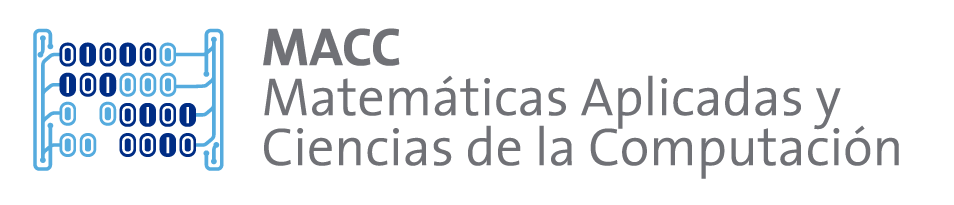
\includegraphics[width=6.5cm]{macc_logo.png}
}
\pagestyle{plain}

\title{Informe de Simulación de Movimiento Planetario}
\author{Isabella Martínez y Camilo Martínez}
\date{\today}


\begin{document}
\maketitle
\thispagestyle{fancy}

\begin{multicols}{2}
	\section{Introducción}
	El movimiento de los planetas ha sido un interrogante desde los orígenes no solo de la ciencia sino también de la humanidad. Importantes avances como los de Galileo Galilei y Johannes Kepler nos permitieron comprender cómo funciona nuestro sistema solar y las leyes que rigen el universo.\\
	
	En esta práctica se pretende simular mediante aproximaciones dadas por métodos numéricos como Euler, Euler-Cromer y Midpoint el movimiento de planetas regidos por la fuerza de gravitación universal de Newton, a su vez que comprobar experimentalmente las leyes de Kepler y analizar la corrección relativista de Albert Einstein.
	
	\section{Marco Teórico}
	La mayoría de nuestro conocimiento sobre la mecánica celeste está resumida en las tres leyes de Kepler, que se enuncian de la siguiente manera:
	
	\begin{enumerate}
		\item Cada planeta se mueve en una órbita elíptica con el sol localizado en uno de los focos de esta elipse.
		\item La velocidad de un planeta aumenta a medida que su distancia al sol disminuye, tal que la línea que une al sol con el planeta recorre áreas iguales en tiempos iguales.
		\item El cociente $ T^{2}/a^{3} $ es el mismo para todos los planetas que orbitan al sol, donde $ T $ es el periodo del planeta y $ a $ es el semieje mayor de su órbita elíptica.
	\end{enumerate}

	Además, la ley de la gravitación universal de Newton establece que una partícula de masa $ M $ atrae a otra partícula de masa $ m $ con una fuerza dada por:
	\begin{align}
		\textbf{F} = -\frac{GMm}{r^{2}}\hat{\textbf{r}} = -\frac{GMm}{r^3}\textbf{r}
	\end{align}
	Donde el vector \textbf{r} se dirige de $ M $ a $ m $. El signo negativo en la ecuación anterior implica que la fuerza es de carácter atractor, es decir, tiende a disminuir la separación $ r $.\\
	
	La energía mecánica de un planeta es entonces:
	\begin{align}
		E = \frac{1}{2}mv^{2} - \frac{GMm}{r}
	\end{align}
	
	En el desarrollo de la simulación se encontró conveniente usar un sistema de unidades donde la magnitud del producto $ GM $ no sea grande ni pequeño. En la descripción de órbitas alrededor del sol es útil usar el semieje mayor de la tierra como unidad de longitud, las llamadas \textit{unidades astronómicas} (AU) definidas como:
	$$ 1 \mathrm{AU}=1,496 \times 10^{11} \mathrm{m} $$
	
	La unidad de tiempo es un año (yr) o $ 3,15 \times 10^{7} \mathrm{s} $. En estas unidades el periodo de rotación de la tierra es $ T = 1 $ y su semieje mayor es $ a = 1 \mathrm{AU} $. Bajo estas condiciones tenemos entonces
	$$ G M=4 \pi^{2} \mathrm{AU}^{3} / \mathrm{yr}^{2} $$
	
	La teoría de la relatividad general de Einstein predice una corrección a la fuerza sobre el planeta que varía como $ 1 / r^{4} $ debido al campo gravitacional débil. El resultado importante es que la ecuación del movimiento para la trayectoria del planeta se escribe como: 
	\begin{align}
		\frac{d^{2} \mathbf{r}}{d t^{2}}=-\frac{G M}{r^{2}}\left[1+\alpha\left(\frac{G M}{c^{2}}\right)^{2} \frac{1}{r^{2}}\right] \hat{\mathbf{r}}
	\end{align}
	
	El método de Euler se definirá como: 
	\begin{align*} 
	x & = x + \frac{dx}{dt} \Delta t \\
	y & = y + \frac{dy}{dt} \Delta t \\ 
	V_{x} & = Vx + \frac{dV_{x}} {dt} \Delta t \\
	V_{y} & = V_{y} + \frac{d V_{y}}{dt} \Delta t \\
	t & = t + \frac {dt } {dt } \Delta t 
	\end{align*}
	
	El método de Euler-Cromer como: 
	\begin{align*}
		V_{x} & = Vx + \frac{dV_{x}} {dt} \Delta t \\
		V_{y} & = V_{y} + \frac{d V_{y}}{dt} \Delta t \\
		x & = x + V_{x} \Delta t \\
		y & = y + V_{y} \Delta t \\ 
		t & = t + \frac {dt } {dt } \Delta t 
	\end{align*}
	
	El método de Midpoint como:
	\begin{align*}
		V_{x} & = Vx + \frac{dV_{x}} {dt} \Delta t \\
		V_{y} & = V_{y} + \frac{d V_{y}}{dt} \Delta t \\
		x & = x + \frac{1}{2}(V_{x} + \frac{dx}{dt})\Delta t \\
		y & = y + \frac{1}{2}(V_{y} + \frac{dy}{dt})\Delta t\\
		t & = t + \frac {dt } {dt } \Delta t 
	\end{align*}
	
	\section{Procedimiento}
	Por conveniencia de la simulación vamos a establecer al sol en el punto $ (0,0) $ y vamos a utilizar la Eq. (1) para ver la fuerza con la que atrae el sol (la masa $ M $) a un planeta arbitrario (la masa $ m $).\\
	
	Note que en la siguiente figura descomponemos la fuerza gravitacional en sus componentes en el eje $ x $ y en el eje $ y $. 
	\begin{Figure}
		\centering
		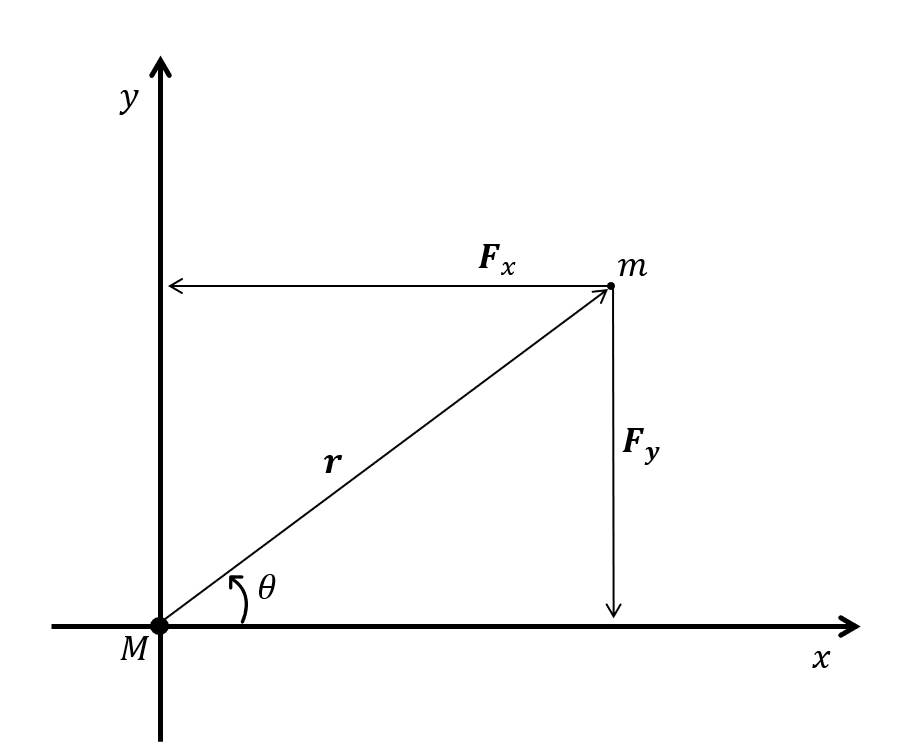
\includegraphics[width=\linewidth]{descomposicion_fuerzas.png}
	\end{Figure}
	Cabe resaltar que entonces $ \cos (\theta) = x / r $ y $ \sin (\theta) = y / r $. Por ende, es conveniente descomponer la fuerza gravitacional en sus componentes en $ x $ y en $ y $ de la siguiente forma:
	
\end{multicols}
	
\end{document}